\documentclass{beamer}
\usetheme{Boadilla}
\usepackage{default}
\usepackage{graphicx}
\graphicspath{ {./images/} }

% fix footer
\makeatother
\setbeamertemplate{footline}
{
	\leavevmode%
	\hbox{%
		\begin{beamercolorbox}[wd=.4\paperwidth,ht=2.25ex,dp=1ex,center]{author in head/foot}%
			\usebeamerfont{author in head/foot}\insertshortauthor
		\end{beamercolorbox}%
		\begin{beamercolorbox}[wd=.6\paperwidth,ht=2.25ex,dp=1ex,center]{title in head/foot}%
			%\usebeamerfont{title in head/foot}\insertshorttitle\hspace*{3em}
			\insertframenumber{} / \inserttotalframenumber\hspace*{1ex}
		\end{beamercolorbox}}%
		\vskip0pt%
	}
	\makeatletter
	\setbeamertemplate{navigation symbols}{}

% add section frames
\AtBeginSection[]{
	\begin{frame}
		\vfill
		\centering
		\begin{beamercolorbox}[sep=8pt,center,shadow=true,rounded=true]{title}
			\usebeamerfont{title}\insertsectionhead\par%
		\end{beamercolorbox}
		\vfill
	\end{frame}
}

\title{Thumbs Up? Sentiment Classification using Machine Learning Techniques}
\subtitle{Pang, Lee, Vaithyanathan - EMNLP 2002}
\author{Slides by: Dor Cohen, Itai Gat}
\institute{IE @ Technion}
\date{\today}
% add github page
\newtheorem{snt}{Review example}
\begin{document}

\begin{frame}
	\titlepage
	Code:
	\centering{http://github.com/dorcoh/sent-emnlp}
\end{frame}




\begin{frame}
	\frametitle{Agenda}
	\tableofcontents
\end{frame}

\section{Introduction}
\subsection{Topic classification}

\begin{frame}
	\frametitle{Topic classification}
	\begin{itemize}
	\item Recent (2002) works sort documents according to their \textbf{subject}
	\begin{itemize}
		\item e.g., sports vs. politics
		\item spam vs. no-spam
	\end{itemize}
	\pause
	\item Yet crucial part of online posted articles is their \textbf{sentiment} (or overall opinion)
	\begin{itemize}
		\item provide useful insights for readers automatically
		\item e.g., product review is negative or positive
	\end{itemize}

	\end{itemize}
\end{frame}

\begin{frame}
	\frametitle{Topic classification}
	\framesubtitle{Current (2002) techniques for non-topic text categorization}
	\begin{itemize}
		\item Source style with features as stylistic variation (Biber, 1988)
		\begin{itemize}
			\item e.g., author, publisher (NY times vs. Daily News)
		\end{itemize}
		\item Genre of text
		\begin{itemize}
			\item e.g., editorial 'subjective' genre
		\end{itemize}
		\item Is subjective language used?
		\item Does text contains opinion expressing?
	\end{itemize}
\end{frame}

\subsection{Sentiment analysis}

\begin{frame}
	\frametitle{Sentiment analysis}
	\begin{itemize}
	\item This work: apply topic classification techniques on sentiment analysis
	\begin{itemize}
		\item Q: What are our expected challenges?
		\pause
		\item A: Topics are identifiable by key words alone, while sentiment requires more \textbf{understanding}
	\end{itemize}
	\end{itemize}
	\pause
	\begin{itemize}
		\item e.g., "How could anyone sit through this movie?"
		\begin{itemize}
			\item Can you mark  any negative word?
		\end{itemize}
	
	\end{itemize}
	\pause
	
	\begin{itemize}
	\item Previous (2002) techniques:
	\begin{itemize}
		\item Semantic orientation of words (Turney and Littman, 2002)
		\item Cognitive linguistic models (Sack, 1994)
		\item Discriminant word lexicons (Tong, 2001)
	
	\end{itemize}
	\end{itemize}
	

\end{frame}

\section{Problem definition}
\subsection{Data}

\begin{frame}
	\frametitle{Problem definition}
	\framesubtitle{Data: IMDB Movie Reviews}
	\begin{itemize}
		\item Lucky for us: user rating provides us \textbf{supervised} learning
		\item Converted into three categories (or topics):
		\begin{itemize}
			\item \emph{Positive}, \emph{negative}, (and \emph{neutral} - not used)
		\end{itemize}
		\item Avoid bias issues:
		\begin{itemize}
			\item 20 reviews per author per sentiment
			\item 752 negative vs 1301 positive
			\item total of 144 reviewers
		\end{itemize}
		\item More preprocess steps: TODO!
	\end{itemize}
\end{frame}

% human based

\subsection{Closer look}
\begin{frame}
	\frametitle{Human based sentiment classifiers}
	\begin{itemize}
		\onslide<1->
		\item In contrast to topics, detecting sentiment is easier for us (why?)
		\begin{itemize}
		
		\onslide<2->
		\item Topics can be related, while with opinions people tend to express strong feelings
		\end{itemize}
		
		\onslide<3->
		\item Hypothesis: certain words indicate on sentiment type
		
		\onslide<4->
		\item Test: decision procedure - count positive vs. negative words
	\end{itemize}
	
	\onslide<5->
	\begin{table}
		\scriptsize
		\begin{tabular}{ l | p{5cm} | c | c }
			Human & Proposed words & Accuracy & Ties \footnotemark \\ \hline \hline
			1 & positive (5): dazzling, brilliant.. \newline negative (5): suck, terrible.. & 58\% & 75\% \\ \hline
			2 & positive (11): gripping, spectacular.. \newline negative (6): cliched, boring.. & 64\% & 39\%  \\  \hline
		\end{tabular}
		\caption{Baseline results for human word lists, data is balanced (700 vs. 700)}
	\end{table}
	
	 \only<5->{\footnotetext{Documents percentage where sentiments rated equally}}
\end{frame}

\begin{frame}
	\frametitle{Human based sentiment classifiers}
	\framesubtitle{Should we worry about high rate of ties?}
	\begin{itemize}
		\item Proposed words list is relatively short (effect is 0 vs. 0 ties)
		\pause
		\begin{itemize}
			\item Not necessarily the reason for low accuracy!
		\end{itemize}
		\pause
		\item Authors propose their own list of words
		\begin{itemize}
			\item Backed up with preliminary \textbf{data analysis} (including test set)
		\end{itemize}
	\end{itemize}
	
	
	\pause
	\begin{table}
		\scriptsize
		\begin{tabular}{ l | p{5cm} | c | c }
			Human & Proposed words & Accuracy & Ties \\ \hline \hline
			3+Stats & positive (7): love, wonderful.. \newline negative (7): bad, worst, '?', '!',.. & 69\% & 16\% \\ \hline
		\end{tabular}
		\caption{Results where words (total 14) were chosen based on data statistics}
	\end{table}
	
	\pause
	Reproduce data analysis (2018), feature occurrences binarized:
	\begin{itemize}
		\small
		\item $\widehat{P(love|d=positive)} = 0.1796$ , $\widehat{P(love|d=negative)} = 0.1334$ \pause
		\item $\widehat{P(worst|d=positive)} = 0.0252$ , $\widehat{P(worst|d=negative)} = 0.0937$
	\end{itemize}
\end{frame}

\section{Methods}
\subsection{Bag of words}

\begin{frame}
\frametitle{Bag of words}

\begin{itemize}
	% introduce unigrams, bigrams
	% relative frequency, tf-idf
	\item $d_1$: "The audio quality really stinks."
	\pause
	\item Extract features:
	\begin{itemize}
		\item Unigrams: \{the,audio,..  \}
		\item Bigrams: \{the audio, audio quality, really stinks,.. \}
		\item N-gram!	
	\end{itemize}
\end{itemize}

\pause
\begin{Definition}[Bag of words framework]
	Let $\{f_1,..f_m\}$ denote set of m features that can appear in document. \\
	Let $n_i(d)$ be the number of times $f_i$ occurs in document $d$. \\ 
	Then each document $d$ is represented by $\overrightarrow{d}:=(n_1(d),...,n_m(d))$.
\end{Definition}

\pause
\underline{Unigram example}
\begin{itemize}
	\item $\overrightarrow{d_1} = (The: 1, audio: 1, quality: 1, really:1, stinks:1)$
	\pause
	\item $d_2$: "Stinking quality, really stinks". \emph{Question:} $\overrightarrow{d_2} = ?$
	\pause
	\item $\overrightarrow{d_2} = (0, 0, 1, 1,2)$
\end{itemize}

\end{frame}

\subsection{Naive bayes}
\begin{frame}
	\frametitle{Naive Bayes classifier}
	\begin{itemize}
		\item Assign class which maximizes probability: $c^{*}=argmax_{c} P(c|d)$
		\pause
		\item Recap:
	\end{itemize}
	
	\begin{Definition}[Bayes theorem]
		\center
		$P(c|d) = \frac{P(c)P(d|c)}{P(d)}$
	\end{Definition}
	\pause
	\begin{itemize}
		\item In practice to estimate $P(d|c)$, we \textbf{naively} assume $f_i$ are conditionally independent.
		\pause
		\begin{itemize}
			\item Hence $\widehat{P(d|c)}=\prod_{i=1}^{m}P(f_i|c)^{n_i(d)}$ 
		\end{itemize}
		\pause
		\item Q: Any numeric issues you can think about?
		\pause
		\item $A_1$: Some estimates are zero, can smooth (e.g., add-one smoothing) 
		\pause
		\item $A_2$: Short documents vs. long documents (propose: tf-idf)
	\end{itemize}
\end{frame}

% add example here
% how to fit nb ?

\subsection{SVM}
\begin{frame}
	\frametitle{Maximum entropy classifier}
	\framesubtitle{aka logistic regression}
	\begin{Definition}[MaxEnt estimator]
		$P(c|d) = \frac{1}{Z(d)} exp(\sum_{i}\lambda_{i,c}F_{i,c}(d,c))$
	\end{Definition}
	\begin{itemize}
		\pause
		\item $Z(d)$ - normalization function
		\pause
		\item $F_{i,c}$ is a \emph{feature/class function}\
		\pause
		\begin{itemize}
			\item Defined: $F_{i,c}(d,c') = 1$ if feature $i$ \textbf{appears} on document $d$ and its estimated class is c, o.w. $F_{i,c}(d,c) = 0$
		\end{itemize}
		\pause
		\item $\lambda_{i,c}$ - feature-weight parameters (large values imply $f_i$ is a strong indicator for class c)
		\pause
		\item Aside: reminds neuron  activation function
	\end{itemize}
	
	\pause
	\underline{Fit procedure}
	\begin{itemize}
		\item Training data used to estimate distribution $F$
		\item $\lambda$'s are set to maximize entropy of induced distribution
	\end{itemize}
			
\end{frame}

\subsection{SVM}
\begin{frame}
	\frametitle{Support vector machines}
	\begin{itemize}
		\item Goal: Find hyperplane $w$ which separates classes with margin large as possible
	\end{itemize}

	\begin{Definition}[SVM hyperplane]
		Let $c_j \in \{1,-1\}$ be the class of document $d_j$ then: \\
		\centering{
		$w:=\sum_{j}\alpha_{j}c_{j}\overrightarrow{d_{j}}$, $\alpha_{j} \geq 0$} \\
	\end{Definition}
	\begin{itemize}
		\item $\alpha_{j}$ are obtained by solving dual optimization problem.
	\end{itemize}
	\pause
	\underline{Alternative fitting procedure:}
	\\
	\begin{Definition}[Gradient descent]
		\centering
		$w = w - \alpha * \frac{\partial L(X,w)}{\partial w} $ , Update till convergence
	\end{Definition}

\end{frame}

\section{Results}
\subsection{Results}

\begin{frame}
	\frametitle{Results and discussion}
	\begin{center}
		\begin{table}
			\begin{tabular}{l | l | l | l || l | l | l}
				ID & Features & count & freq/pres & NB & ME & SVM \\ \hline \hline
				1 & unigrams & 16165 & freq & 78.7\% & NA & 72.8\% \\
				2 & unigrams & 16165 & pres & 81.0\% & 80.4\% & \textbf{82.9}\% \\
			\end{tabular}
			\caption{3-fold average accuracies, unigrams appear at least 4 times on corpus.}
		\end{table}
	\end{center}
	\pause
	\begin{itemize}
		\item Recall human baseline ranges between $50\%-69\%$ \pause
		\item Topic-based classification reached $90\%+$ accuracy \pause
		\begin{itemize}
			\item Settings were multi-class
			\item We conclude that sentiment analysis is harder
		\end{itemize} \pause
		\item The frequency vs. presence of features seems to make the difference \pause
		\begin{itemize}
			\item Hence from this point authors use presence (\textbf{binarized occurrences})
		\end{itemize}
	\end{itemize}
\end{frame}

\begin{frame}
	\frametitle{Results and discussion}
	\framesubtitle{Using feature presence}
	\begin{center}
		\begin{table}
			\begin{tabular}{l | l | l || l | l | l}
				ID & Features & count & NB & ME & SVM \\ \hline \hline
				2 & unigrams & 16165 & 81.0\% & 80.4\% & \textbf{82.9}\% \\
				3 & uni+bigrams & 32330 & 80.6\% & 80.8 & \textbf{82.7}\% \\
				4 & bigrams & 16165 & 77.3\% & 77.4\% & 77.1\% \pause \\ \hline \hline
				5 & unigrams+POS & 16695 & 81.5\% & 80.4\% & \textbf{81.9}\% \pause \\
				6 & adjectives & 2633 & 77.0\% & 77.7\% & 75.1\% \pause \\
				7 & top 2633 unigrams & 2633 & 80.3\% & 81.0\% & 81.4\% \pause \\
				8 & unigram+position & 22430 & 81.0\% & 80.1\% & \textbf{81.6}\% \\
			\end{tabular}
			\caption{3-fold average accuracies, bigrams appear at least 7 times on corpus.}
		\end{table}
	\end{center}
	\pause
	\begin{itemize}
		\item Adding bigrams doesn't improve results; Bigrams alone is worse \pause
		\item Part-of-speech: "I love this movie" vs. "This is a love story" \pause
		\item Position based on dividing text into quarters.
	\end{itemize}
\end{frame}

\section{Reproduce results}
\begin{frame}
	\frametitle{Reproduce results}
	\framesubtitle{(2018)}
	\begin{itemize}
		\item We have tried to reproduce the experiment for the best settings reported
	\end{itemize}
	\begin{center}
		\begin{table}
			\begin{tabular}{l | l | l || l | l | l}
				Features & count & NB & ME & SVM & MLP\\ \hline \hline
				unigrams & 16165 & 81.0\% & 80.4\% & \textbf{82.9}\% & NA \pause \\
				unigrams & 16165 & 77.48\% & \textbf{81.52}\% & 48.19\% & \textbf{82.75}\%  \\
			\end{tabular}
			\caption{Original vs. our results}
		\end{table}
	\end{center} \pause
	\begin{itemize}
		\item \textbf{No tuning} was used at all; Plus not all described processing steps applied 
		\item Notebook is available here(link)
	\end{itemize}
\end{frame}

\begin{frame}
	\frametitle{Classifier comparison}
	\framesubtitle{(2018)}
	\begin{itemize}
		\item Let's observe our classifiers decision boundaries for some toy datasets: \pause
	\end{itemize}
	\begin{center}
		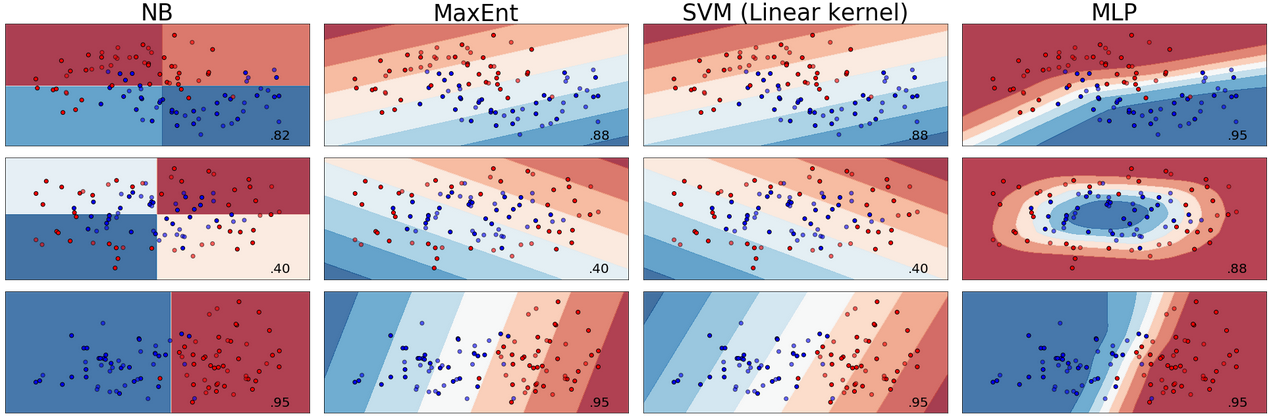
\includegraphics[scale=0.26]{comparison}
	\end{center}
	
\end{frame}

\section{Conclusions}
\begin{frame}
	\frametitle{Conclusions}
	\begin{itemize}
	\item Unigrams presence setting achieves the best performance \pause
	\item Applying selection algorithms for unigrams could improve performance \pause
	\item Contrarily, performance isn't comparable to topic classification 
	\end{itemize}
	\pause

	\begin{snt}
		"This film should be brilliant. It sounds like a great plot, the actors are first grade, and the supporting cast is good as well, and Stallone is attempting to deliver a good performance. However, it can't hold up."
	\end{snt}
	\pause
	
	\begin{itemize}
		\item Difficult for bag-of-words classifiers. \pause
		\item Authors suggest determining the \textbf{focus} of each sentence, if is on/off topic.
	\end{itemize}
\end{frame}

\begin{frame}
	\centering
	\huge
	Thank you for participating! \\
	Questions?
\end{frame}

\end{document}
